
\chapter[]{Modularisation des systèmes distribués}% TODO: maybe rename.
%%% - Programme/Processus
%%% - Exécutable

Les programmes modernes ont une structure \textit{modulaire},
c'est-à-dire que leur code se décompose logiquement en différentes
parties relativement indépendantes, les \textit{modules}.  Cette
structure a de nombreux avantages, entre autres sur le plan du
développement et de la maintenance.  La structure d'un programme en
vue de son \textit{déploiement} -- c'est-à-dire comment son code
exécutable est stocké sur disque, chargé en mémoire, etc. -- peut prendre
plusieurs formes.

Un programme sous forme \textit{monolithique} contient dans son code exécutable
toutes les instructions exécutées par l'ordinateur.  Cette forme était la norme
dans les premiers systèmes informatiques, et l'est toujours pour les systèmes
embarqués qui n'ont pas de système d'exploitation indépendant.  Lorsqu'un
système d'exploitation est disponible sur l'ordinateur on peut le considérer
comme étant un module puisqu'il offre des services précis avec une interface
standardisée.  Dans ce cas, un programme peut prendre la forme d'un seul
fichier de code qui, à son exécution, communiquera avec le système
d'exploitation pour accéder à ses services.  Ce genre de fichier exécutable est
obtenu par une \textit{édition de liens statique} qui combine en un seul
fichier tous les modules (à l'exception du système d'exploitation).  Par
rapport à la forme monolithique, cette organisation simplifie le développement
car le programmeur n'a pas à se soucier du développement des services de base
comme l'accès aux fichiers, la gestion des processus et de la mémoire, etc.  Le
programme peut être distribué à d'autres ordinateurs ayant le même système
d'exploitation simplement en y transférant le fichier exécutable.

L'édition de lien statique a un certain nombre de défauts. La version des
modules utilisé au moment de l'édition de liens est figée au sein du
programme, ce qui empêche la mise à jour individuelle des modules. Il faut
recompiler tous les modules qui ont subi une mise à jour et refaire l'édition de liens du
programme principal. Le coût en temps et l'effort pour un changement minime
est important.  Le chapitre \ref{ch:loading-model} va détailler plus en profondeur
ces problèmes.

% Le même module est chargé plus d'une fois.
L'édition de liens peut se faire paresseusement par le système d'exploitation à
l'exécution du programme, ce qu'on appelle l'\textit{édition de liens dynamique}.  Cela
permet de garder la structure modulaire au \textit{déploiement}.
Chaque module est une composante séparée du programme principal.  Ces modules
sont lu du disque et chargés en mémoire durant l'exécution du programme.  Ce
chargement est effectué par \textit{éditeur de liens dynamique} qui s'occupe de
lié les fonctionnalités des modules au programme principal. Le chapitre % chapter or section
\ref{ch:loading-model} explique plus en profondeur le fonctionnement de éditeur de liens
dynamique. L'avantage principal du chargement dynamique de module est la mise à jour
individuelle d'un module sans avoir a lié le programme principale; dans le
modèle statique le programme principal doit être lié à nouveau avec les modules.
Les modules chargés dynamiquement par le système d'exploitation peuvent être partagé entre différent
programme. Ce type de module porte le nom de \textit{bibliothèque partagée} ils sont décrit dans
le chapitre \ref{ch:loading-model}.

% % Migration de code dans un système distribué.
% - Transmission de tâche entre des machines d'un système distribué.
%   - Un module absent sur la machine distante nécessaire à l'exécution
%   de la tâche transmise.
%     - Télécharger le module d'un serveur dédié.
%     - Revient au chargement dynamique de ce module.

Un programme distribué est séparé sur plusieurs systèmes. Dans un système
distribué, il est possible de transmettre des tâches entre les différents
systèmes. C'est ce qu'on appelle, \textit{migration de tâche}.  Un exemple de
migration de tâche est l'invocation de \texttt{ssh} qui permet d'exécuter un
processus sur un système distant. Le problème de cette approche est que le
programme doit exister sur la machine distante et que chaque invocation passe
par une authentification. Des mécanismes de migration de code ont été
implémentés dans différents langages comme Erlang~\cite{M_mobileintelligent},
Java~\cite{And98transparentmigration}, Scheme~\cite{Sumii00animplementation},
Javascript~\cite{DEV2017transparentmigration}, \dots.  La plupart des méthodes
de migration de code requièrent que l'ensemble des procédures sont
présentes sur le système distant.

Le système Java~\cite{And98transparentmigration} capture l'état du programme courant
qui consiste aux valeurs et aux types de toutes les variables de chaque objet. L'autre
information est la pile des appels de méthode avec les valeurs de toutes les variable.
Ces informations sont transmis et utilisés pour reconstruire l'état du programme.
L'ensemble des méthodes sur le nœud de départ est présent sur le nœud d'arrivé.
Le système Erlang~\cite{M_mobileintelligent} requière aussi que le code soit disponible
sur le nœud destination.

Le système de migration en Javascript utilise des dépôts de code pour
conserver le code. Il est basé sur le fait que le code des agents
sont connus. Puisque le code des agents est connu, il suffit de transmettre
l'état de l'agent. Ce modèle Javascript ressemble à celui implémenté dans
dans Gambit.

La migration de de code ne devrait pas être limité par le code sur le nœud
distant. Le système de module offre la possibilité de migrer un agent sur un
nœud qui ne connait pas le code de l'agent. Un exemple concret de migration
de code est présenté dans le chapitre \ref{ch:task_migration}.


% \section{Linkage statique}
% Cette forme d'édition de lien permet la création de binaire qui indépendant
% qui facilite le déploiement.

%\section{Linkage dynamique}

--------------------------END---------------------------

% TODO: move to chapter task_migration
Un programme sur une des machine du système distribué qui se fait transmettre
une tâche peut devoir exécuter une fonctionnalité d'un module absent
localement. Cela nécessite un téléchargement du module contenant la
fonctionnalité demandé d'un serveur dédié. Une fois le module installé, il faut
le charger dynamiquement.

==> motiver (quels problèmes ça cause le link statique) et expliquer le chargement dynamique, système distribué, etc
% TODO lien => liens


%Problème du link statique\\
% - Gèle les versions des modules au sein du programme. \\
%    -> Comment la maintenance d'un programme lié statiquement? \\
%    - Le temps de compilation. (Coût d'un changement est important) \\
% - La taille du programme peut être plus importante.
% - Le même module est chargé plusieurs fois en mémoire.

--------------------------------------------------------


Dans les systèmes comme DOS, les programmes ou modules devaient contenir toutes les
informations nécessaire pour s'exécuter. De tels programmes sont dit lié
statiquement dans le sens qu'il ne dépende que de l'architecture sur laquelle il
a été construit. La construction des modules requière deux étapes. La compilation
de fichier source en fichier objet contenant le nom et le code des fonction.
L'édition des liens qui réunit un plusieurs fichiers objets en un module.
Dans le cas d'un seul fichier l'édition des liens ne fait que transformer le fichier
objet en fichier exécutable.

\begin{figure}[ht]
  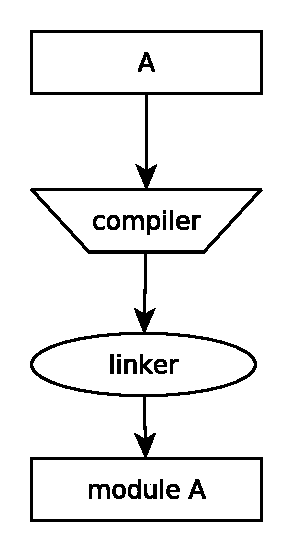
\includegraphics[width=0.20\linewidth]{figures/basic_module_compilation.pdf}
  \caption{Construction du module A à partir des sources.}
\end{figure}

%La création d'exécutable inclut deux étapes importantes, la compilation et
%l'édition des liens. La première étape consiste à prendre un fichier de code
%source et de le traduire en fichier objet, que l'on retrouve souvent avec
%l'extension \verb|.o| ou \verb|.obj|, qui contient la représentation des
%procédures compréhensible par le processeur. Ces fichiers objets ne sont pas
%encore exécutable pour autant, il faut tout d'abord effectuer la seconde étape,
%qui va les regrouper en un exécutable. Le programme qui s'occupe de l'édition
%des liens est le \textit{linker}, la version GNU se nomme \verb|ld|.  Voici
%l'exemple de la création d'un exécutable composé des fichiers sources C
%\verb|main.c| et \verb|foo.c|:
%
%\begin{figure}[ht]
%    \begin{minipage}[t]{0.5\textwidth}
%\begin{verbatim}
%# Compilation
%gcc -c main.c -o main.o
%gcc -c foo.c -o foo.o
%# Édition de liens
%ld -o main.exe main.o foo.o
%\end{verbatim}
%    \end{minipage}
%
%    \caption{Exemple de création d'un exécutable}
%\end{figure}


La construction d'un programme peut s'effectuer de façon modulaire; chaque
composantes du programme peuvent être construites en séparément.  La
modification d'une des bibliothèques partagés utilisés par
le programme ne nécessite pas la recompilation de celui-ci. Le nom qui est
donné à l'entité qui résout les noms des fonctionnalités est l'éditeur de liens (\textit{dynamic linker}).
Habituellement les bibliothèques exportent des fonctions, mais il peuvent aussi
exporter plusieurs types de données comme des entiers, des nombres à virgules,
des chaînes de caractères et des données composites (structures). Chacune de ces données est
associées à un nom unique (symbole) au sein de la bibliothèque.
Il n'est pas possible d'avoir deux bibliothèques statiques qui exportent une
fonctionnalité avec le même nom au sein d'une même application, alors qu'avec
les bibliothèques partagés c'est possible. Cela limite le choix des
bibliothèques qui peuvent être utilisé simultanément au sein du programme;
chaque bibliothèque doit avoir un ensemble de nom de fonctionnalité distinct
des autres. Puisque la résolution d'une fonctionnalité retourne la première
occurrence trouvée, il n'y a rien qui empêche d'avoir plus d'une fonctionnalité
associée au même nom.

Gambit permet de l'utilisation de bibliothèques statiques et dynamiques.
Chaque fichier Scheme peuvent être compilé et lié module exécutable ou
en bibliothèque dynamique.

\begin{center}
\begin{figure}[ht]
  \begin{tabular}{l}
    \begin{mplisting}{0.5}
;; fib.scm
(define (fib n)
  (if (< n 2)
      n
      (+ (fib (- n 1))
         (fib (- n 2)))))
\end{mplisting}
  \end{tabular}
  \caption{Un module qui implémente la fonction mathématique \texttt{fib}.}
  \label{fig:basic_fib_module}
\end{figure}
\end{center}

\vspace{-20pt}
La construction d'un bibliothèque dynamique à partir du fichier \texttt{fib.scm}
de la figure \ref{fig:basic_fib_module} s'effectue par le compilateur de Gambit
qui nomme \texttt{gsc}. Cela produit un fichier avec l'extension \texttt{.oN}
où le \texttt{N} correspond à la version généré de la bibliothèque qui commence à 1.


\section{Concepts}

% Définition sommaire d'une bibliothèque de code
Une bibliothèque de code est le regroupement de plusieurs types
de données, des entiers, des nombres à virgule flottant, des chaînes
de caractères, des fonctions et des données composites. L'ensemble
de ces données constitue les fonctionnalités de la bibliothèque.
Les fonctionnalités d'une bibliothèque peut être copié dans l'exécutable
(bibliothèque statique), cela facilité la distribution du binaire puisque
que ses dépendances sont inclus dans l'exécutable.
Les fonctionnalités d'une bibliothèque peuvent aussi être chargé
à l'exécution (bibliothèque partagés), cela permet de partagé des routine
commune entre plusieurs processus (programme en exécution). Les données de
la bibliothèque, par contre, ne sont partagé, chaque processus réfère à
sa propre version des données.
Le format d'une bibliothèque de code varie d'un langage à l'autre et aussi d'un
système d'exploitation à un autre. Les langages interprétés utilisent plus
souvent le code source directement ou une représentation intermédiaire comme format pour
les bibliothèques de code.
Pour les langages compilés, c'est le format natif correspondant au système d'exploitation
qui est le plus souvent utilisé. Le système d'exploitation Linux utilise le
format ELF (Extensible Linking Format), Microsoft Window utilise le format PE (Portable Executable)
et MacOSX utilise le format Mach-O (Mach object) pour les exécutables et les bibliothèques.
% XXX: bytecodes aussi pour les langage compilé.

%Les langages
%de programmation interprétés fournisse leurs bibliothèques directement
%en code source. Dans cette catégorie, il y a Ruby, Python, Perl, Lua et
%Scheme -- dont le code des bibliothèques est écrit et frounit dans le
%langage respectif. Les langages compilés -- comme C, C++, C\# et Java --
%utilisent plutôt des formats binaires destiné, soit à une machine virtuelle
%(e.g. la \textit{Java Virtual Machine} JVM ou un architecture
%physique (e.g. i686, x86\_64, ARM). Les bibliothèques natives peuvent
%être utilisé




Une application qui utilise une bibliothèque partagés ne contient pas le
code de la bibliothèque, mais plutôt le nom des fonctionnalités utilisés.
La routine qui permet de récupérer la fonctionnalité
à partir du nom est la résolution qui est effectué par le \textit{dynamic loader}.
Lorsqu'un programme lié dynamiquement
à plusieurs bibliothèques partagés exécute du code externe \verb|foo|,
un routine de résolution est démarré pour déterminé quelle bibliothèque
lié au fournit la fonctionnalité \verb|foo|.

%% Bibiothèque dynamique native.
Par exemple, sous Linux l'utilitaire <<yes>>, qui est écrit en C,
est lié aux bibliothèques systèmes suivantes:
\begin{verbatim}
  linux-vdso.so.1 (0x00007ffeef7f9000)
  libc.so.6 => /usr/lib/libc.so.6 (0x00007ff68161c000)
  /lib64/ld-linux-x86-64.so.2 => ...
\end{verbatim}
La bibliothèque \textit{libc.so.6} contient la plupart des fonctions
standards du système sous Linux dont les fonctionnalités sont résolut
à l'exécution.
% Le but d'une bibliothèque est la réutilisation de code.
Dans le contexte d'un exécutable natif, le chargement des bibliothèques
s'effectue au début de l'application, avant l'exécution de la fonction principale
souvent nommé \textbf{main}. Plusieurs bibliothèques peuvent coexister simultanément au
sein d'un même processus sans que l'exécution du programme en soit affecté.

La résolution des fonctionnalité de ces bibliothèques sont effectué par un programme adapté
le \textit{program interpreter} du système qui correspond à \textit{/lib64/ld-linux-x86-64.so.2}.
Il est possible de forcer la résolution d'une fonctionnalité d'une bibliothèque
de façon manuel. Ce genre d'interaction est possible sur
les trois principales plateformes utilisées sur le marché (Windows, MacOSX et Linux).

%% TODO: continue here FIXME
Sur Linux, l'API qui permet d'interagir avec les bibliothèques partagés provient de \textit{libdl.so}.
Elle contient les fonctions \textit{dlopen}, \textit{dlsym}, \textit{dlerror} et \textit{dlclose} pour gérer
des bibliothèques de code supplémentaire chargé manuellement à l'exécution.  Pour charger la fonction
\textit{foo}, qui ne prend pas d'argument et ne retourne rien de la bibliothèque \textit{libFoo.so} en C,
il faut exécuter les deux appels suivant:
\begin{center}
  \begin{figure}[ht]
\begin{lstlisting}[language=C,frame=single]
  ...
  void *handle = dlopen("./libFoo.so", RTLD_LAZY);
  void (*foo)() = dlsym(handle, "foo");
  ...
\end{lstlisting}
\caption{Chargement dynamique de la bibliothèque \textit{libFoo.so} et
résolution de la fonction \textit{foo} sans gestion d'erreur sous Linux}
  \end{figure}
\end{center}
L'équivalent des bibliothèques partagés sous Window sont les DLLs, ils peuvent être chargé de façon similaire dans un
programme en utilisant les fonctions \textit{LoadLibrary}, \textit{LoadLibraryEx} et \textit{GetProcAddress}. Ils
fonctionne de la même façon que leur équivalent Linux. Pour MacOSX, il faut passer par les routines:
\begin{itemize}
    \item \textit{NSCreateObjectFileImageFromFile}
    \item \textit{NSLinkModule}
    \item \textit{NSLookupSymbolInModule}
    \item \textit{NSAddressOfSymbol}
\end{itemize}

La majorité des langages interprétés permettent l'importation de bibliothèque de code natif, via un interface
nommé \textit{foreign function interface}.
Prenons comme exemple les langage Python, Ruby, Lua et Scheme. Python possède le module ctypes
qui permet de chargé des bibliothèques natives dynamique, Ruby possède le module ffi.
%Ces modules ne font qu'encapsuler les fonction de chargement de bibliotheques native pour qu'il puisse être invoqué
%dans le langage cible.

% Bibliothèque Lua en C
% - La bibliothèque doit avoir le même nom que celui utilisé par le \textit{import}.

Certains langages ont même un mécanisme pour charger des bibliothèques natives s'ils ont été conçus spécialement.
Dans le langage de programmation Lua, il est possible en Lua de chargé directement
une bibliothèque dynamique si elle contient une fonction principale \textbf{luaopen\_\textit{libname}}
où \textit{libname} est le nom de la bibliothèque.

Gambit Scheme utilise un mécanisme équivalent. Il permet le chargement de ces modules qui ont été compilé
en bibliothèque partagé (DLL) avec la fonction \textit{(\textbf{load} "libname")}. Le chargements de la
bibliothèque ressemble à celui de Lua.

%% Python
%\begin{figure}[ht]
%\begin{lstlisting}[language=python,frame=single]
%# From https://docs.python.org/2/library/ctypes.html
%from ctypes import *
%# Chargement d'une bibliotheque native.
%lib = cdll.LoadLibrary("./libFoo.so")
%# Appel de la fonction foo.
%lib.foo()
%\end{lstlisting}
%\caption{Code d'importation de la fonction \textbf{foo} de la bibliothèque \textit{libFoo.so} en Python}
%\end{figure}

\begin{center}
% Ruby
\begin{figure}[ht]
\begin{lstlisting}[language=ruby,frame=single]
require 'ffi'
# Chargement d'une bibliotheque native.
module LibFoo
    extend FFI::Library
    ffi_lib './libFoo.so'
    attach_function :foo, [], :void
end
# Appel de la fonction foo.
LibFoo.foo
\end{lstlisting}
\caption{Code d'importation de la fonction \textbf{foo} de la bibliothèque \textit{libFoo.so} en Ruby}
\end{figure}
\end{center}

La résolution des fonctionnalités effectué par le \textit{dynamic linker} utilise un ordre de recherche
définit. Cet ordre de recherche inclut l'exécutable courant, les dépendances de l'exécutable, la bibliothèque
passé à \textit{dlsym}. La résolution d'une fonctionnalité par \textit{dlsym} qui n'engendre pas la résolution
d'un autre fonctionnalité externe n'utilise pas le programme principale dans l'ordre de recherche qui alors
commence par la bibliothèque passé à \verb|dlsym| suivit de ses dépendances. Les résolution de fonctionnalité
provenant d'appels indirecte au \textit{dynamic linker} inclut le programme principal et ses dépendances avant
la bibliothèque passé à \verb|dlsym|.

\begin{center}
    \begin{figure}[ht]
        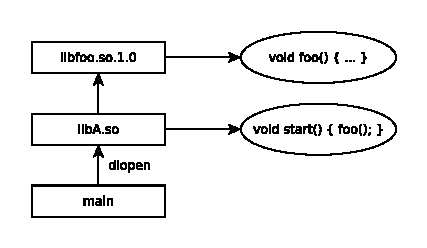
\includegraphics{figures/libdeps-ex1.pdf}
        \caption{Un exemple de dépendance de bibliothèques au sein d'un application simple fictive.
            La bibliothèque \textit{libA.so} est chargé dans l'application \texttt{main} via
            les appels au procédure \textit{dlopen} et \textit{dlsym}. Le fonctionnalités utilisés
            dans l'exemple sont marqué par un ellipse.
        }
        \label{fig:deps-ex1}
    \end{figure}
\end{center}

Dans la situation situation présenté dans la figure-\ref{fig:deps-ex1}, quels sont les étapes inclut
dans l'exécution de ce programme qui ne fait qu'appeler la fonctionnalité \texttt{start} de la
bibliothèque \textit{libA.so}. La fonctionnalité \texttt{start} est résolu de façon direct par
un appel à \verb|dlsym(libA, "start")|, qui commence la recherche de la procédure \texttt{start} dans
la bibliothèque spécifier dans \texttt{dlsym}. Le programme, une fois la procédure trouvé, l'exécute.
L'appel à une procédure non résolue (e.g.\ la procédure \texttt{foo} invoqué dans \texttt{start})
déclenche une procédure automatique de résolution des fonctionnalités. Cette procédure de résolution
commence sa recherche à partir de l'exécutable, puis itère la liste des dépendances directe. Si la
fonctionnalité n'est pas encore trouvé, la recherche continuera à partir de la bibliothèque passé à
\texttt{dlsym}.

% Stub

% TODO: exemple de résolution direct
Connaissant l'ordre de recherche du \textit{dynamic linker}, il est facile de construire un application avec des bibliothèques
qui cause un masquage de fonctionnalité. Deux possibilité facilement exploitable, faire que l'exécutable main fournisse
directement la fonctionnalité à masquer, ou avoir une des dépendances de l'exécutable contenant cette fonctionnalité. La figure-\ref{fig:deps-ex2}
en est l'exemple qui utilise la seconde méthode. La première consisterait à transformer l'exécutable main est bibliothèque
exécutable qui ne pourrait pas être supporté sur certaine plateforme. Sous Linux, il est possible de créer une bibliothèque qui
exécutable en passant le paramètre \texttt{-rdynamic} à \textit{gcc} lors de la construction.

\begin{center}
    \begin{figure}[ht]
        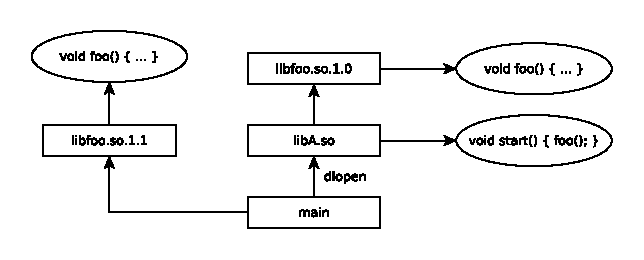
\includegraphics{figures/libdeps-ex2.pdf}
        \caption{Exemple de dépendance dans un application cause le masquage de la fonctionnalité \texttt{foo}
        de la bibliothèque \textit{libfoo.so.1.0} par la bibliothèque \textit{libfoo.so.1.1}}
        \label{fig:deps-ex2}
    \end{figure}
\end{center}
%% BEGIN
% D'autre langage compilé comme C/C++
% ne le permette pas directement, la liste des bibliothèques de code utilisé par un
% programme est déterminée lors de la création du fichier binaire, qui peut être
% soit un exécutable où une bibliothèque.
%% END


% TODO: pourquoi est-ce utile?
% XXX: structure pas final.
% - Les bibliothèques coexistent dans les application de tous les jours.
Analyser les interactions entre des bibliothèques au sein d'un même programme permet de
mieux comprendre quels sont les circonstance qui peuvent conduire à des comportements
non désirés, par exemple le masquage démontré dans la figure-\ref{fig:deps-ex2}.
Cela permet aussi d'établir les conditions qui inhibe ces comportements non désirés.

%Cela implique que ils possible de retrouvé une dépendance en diamant tel que représenter
%dans la figure-\ref{fig:dep1} qui peut causer un problème. % Détailler
%\begin{figure}[ht] %% Pas juste valide pour scheme.
%  \begin{center}
%    %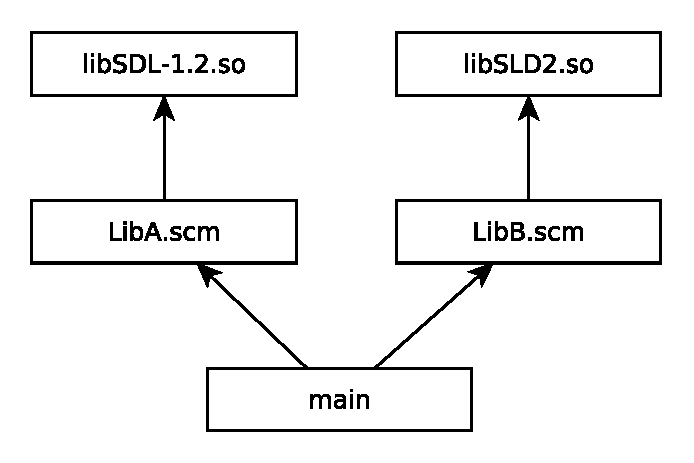
\includegraphics[width=4cm]{figures/SchemeLibrary}
%    \caption{Dépendence en diamant}
%    \label{fig:dep1}
%  \end{center}
%\end{figure}

%% NOTE: Soit P un processus, execution(A, P=[A,B]) == execution(A, P=[A]).
%Soit un processus \textbf{P} qui réfère aux bibliothèques \textbf{A} et \textbf{B}.
%Une bibliothèque peut masquer les symboles d'une autre bibliothèque chargé dans le même processus.
%La bibliothèque \textbf{A} coexiste avec la bibliothèque \textbf{B} si la \textbf{A}
%ne masque pas des symboles ne \textbf{B} qui amène un comportement non défini.


% Historiquement, il y avait un problème avec la coexistence entre deux dll sous Window. TODO: devellopper

% - Système distribué (Actor), non limité par la diversité des bibliothèque.


% TODO:
%La coexistance entre plusieurs versions d'une même bibliothèque
%===========================================================
%
% - Définition d'une bibliothèque
%   - Nom symboles:
%     - Fonction
%     - Variables global
%     - Structure de donnée
%     - Macro (Compilation)
%
%- Définition par coexistence de plusieurs bibliothèque.
%- Pourquoi est-ce utile?
%- Conditions nécessaire pour la coexistence entre plusieurs versions d'une même bibliothèque soit possible.
%  - Data race.
%  - État partagé.
%- Système d'exploitation (DOS)


